%%%%%%%%%%%%%%%%%%%%%%%%%%%%%%%%%%%%%%%%%%
% Short Sectioned Assignment LaTeX Template Version 1.0 (5/5/12)
% This template has been downloaded from: http://www.LaTeXTemplates.com
% Original author:  Frits Wenneker (http://www.howtotex.com)
% License: CC BY-NC-SA 3.0 (http://creativecommons.org/licenses/by-nc-sa/3.0/)
%%%%%%%%%%%%%%%%%%%%%%%%%%%%%%%%%%%%%%%%%

%----------------------------------------------------------------------------------------
%	PACKAGES AND OTHER DOCUMENT CONFIGURATIONS
%----------------------------------------------------------------------------------------

\documentclass[paper=a4, fontsize=11pt]{scrartcl} % A4 paper and 11pt font size

% ---- Entrada y salida de texto -----

\usepackage[T1]{fontenc} % Use 8-bit encoding that has 256 glyphs
\usepackage[utf8]{inputenc}
%\usepackage{fourier} % Use the Adobe Utopia font for the document - comment this line to return to the LaTeX default

% ---- Idioma --------

\usepackage[spanish, es-tabla]{babel} % Selecciona el español para palabras introducidas automáticamente, p.ej. "septiembre" en la fecha y especifica que se use la palabra Tabla en vez de Cuadro

% ---- Otros paquetes ----

\usepackage{url} % ,href} %para incluir URLs e hipervínculos dentro del texto (aunque hay que instalar href)
\usepackage{amsmath,amsfonts,amsthm} % Math packages
%\usepackage{graphics,graphicx, floatrow} %para incluir imágenes y notas en las imágenes
\usepackage{graphics,graphicx, float} %para incluir imágenes y colocarlas

% Para hacer tablas comlejas
%\usepackage{multirow}
%\usepackage{threeparttable}

%\usepackage{sectsty} % Allows customizing section commands
%\allsectionsfont{\centering \normalfont\scshape} % Make all sections centered, the default font and small caps

\usepackage{fancyhdr} % Custom headers and footers
\pagestyle{fancyplain} % Makes all pages in the document conform to the custom headers and footers
\fancyhead{} % No page header - if you want one, create it in the same way as the footers below
\fancyfoot[L]{} % Empty left footer
\fancyfoot[C]{} % Empty center footer
\fancyfoot[R]{\thepage} % Page numbering for right footer
\renewcommand{\headrulewidth}{0pt} % Remove header underlines
\renewcommand{\footrulewidth}{0pt} % Remove footer underlines
\setlength{\headheight}{13.6pt} % Customize the height of the header

\numberwithin{equation}{section} % Number equations within sections (i.e. 1.1, 1.2, 2.1, 2.2 instead of 1, 2, 3, 4)
\numberwithin{figure}{section} % Number figures within sections (i.e. 1.1, 1.2, 2.1, 2.2 instead of 1, 2, 3, 4)
\numberwithin{table}{section} % Number tables within sections (i.e. 1.1, 1.2, 2.1, 2.2 instead of 1, 2, 3, 4)

\setlength\parindent{0pt} % Removes all indentation from paragraphs - comment this line for an assignment with lots of text

\newcommand{\horrule}[1]{\rule{\linewidth}{#1}} % Create horizontal rule command with 1 argument of height






%----------------------------------------------------------------------------------------
%	TÍTULO Y DATOS DEL ALUMNO
%----------------------------------------------------------------------------------------

\title{	
\normalfont \normalsize 
\textsc{\textbf{Grundlagen der Wissensverarbeitung} \\ Computer Science \\ Universität Hamburg} \\ [25pt] % Your university, school and/or department name(s)
~\\
~\\
~\\
\horrule{0.5pt} \\[0.4cm] % Thin top horizontal rule
\Huge Übung 1: Search Space Design \\ % The assignment title
\horrule{2pt} \\[0.5cm] % Thick bottom horizontal rule
~\\
~\\
}

\author{Rafael Ruz Gómez\\Miguel Robles Urquiza} % Nombre y apellidos

\date{\normalsize 5 November 2017} % Incluye la fecha actual

%----------------------------------------------------------------------------------------
% DOCUMENTO
%----------------------------------------------------------------------------------------

\begin{document}

\maketitle % Muestra el Título

\begin{figure}
	\centering
	
\includegraphics[scale=0.8]{logo_uni_hamburg.png}
\end{figure}

\newpage %inserta un salto de página




%----------------------------------------------------------------------------------------
%	Question 1
%----------------------------------------------------------------------------------------

\huge{ \textbf{Exercise 4.3}}
\newline

\large{\textbf{Provide example mazes that show the differences between and properties of the search strategies. Describe these properties}}\\

Breadth first is useful when you want a solution containing the fewest arcs. It's obvious that bread first search have few arcs than depth first search.\\

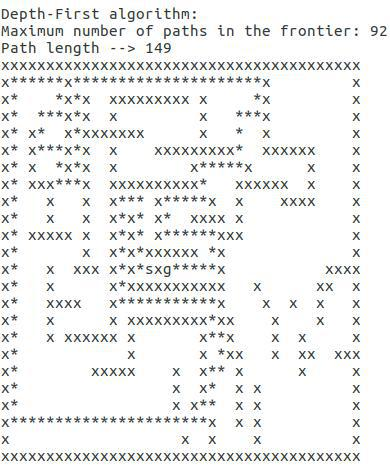
\includegraphics[scale=0.7]{K1.jpg}
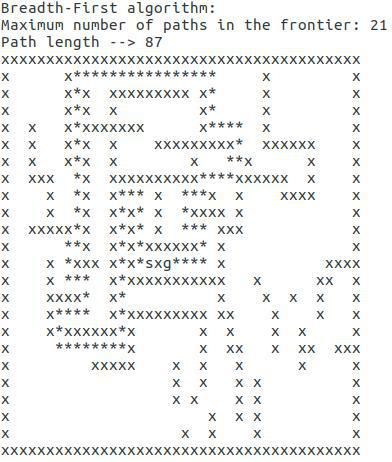
\includegraphics[scale=0.699]{K2.jpg}

%----------------------------------------------------------------------------------------
%	Question 2
%----------------------------------------------------------------------------------------
\newpage
\huge{ \textbf{Exercise 4.4}}
\newline

\large{\textbf{Are there cases in which your program is unable to find a solution? Provide example mazes.}}\\

We have found just one case in wich our program is unable to find a solution, when there is no real solution. We meant, when we can not arrive to the goal because the goal is totally surrounded by 'x'.\\

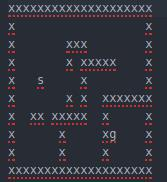
\includegraphics[scale=1.3]{maze.jpg}


%----------------------------------------------------------------------------------------
%	Question 3
%----------------------------------------------------------------------------------------

\huge{ \textbf{Exercise 5.2}}
\newline

\large{\textbf{Write a second heuristic function that works correctly with portals. What do you have to change?}}\\

We check which distance is the minimum distance between our actual position and each portal. If taking this portal we arrive to the goal with minimum cost, we choose this path.\\




%----------------------------------------------------------------------------------------
%	Question 4
%----------------------------------------------------------------------------------------
\newpage

\huge{ \textbf{Exercise 5.3}}
\newline

\large{\textbf{The maze above is a slightly modified version of the environment (Not possible path between start and goal). How does your search react in this case? Can you ensure termination?}}\\

We send a message to the user telling that the program has been unable to find a path between the start node the goal node.\\
Yes, we can ensure termination
\newline

%----------------------------------------------------------------------------------------
%	Question 5
%----------------------------------------------------------------------------------------

\huge{ \textbf{Exercise 5.4}}
\newline

\large{\textbf{For each of the search strategies used so far document the time and memory resources used by the algorithm in terms of expansion operations performed on the frontier of the search and the maximal number of nodes in the frontier.}}





\newpage
%------------------------------------------------

%\bibliography{citas} %archivo citas.bib que contiene las entradas 
%\bibliographystyle{plain} % hay varias formas de citar

\end{document}

